\newpage
\section{Resultaten}
In deze sectie tonen en bespreken we de bekomen resultaten.

\subsection{Aantal Snijpunten}
\begin{figure}[H]
   	\centering
   	\includegraphics[width=\textwidth]{illustraties/3DnrIs.png}
  	\label{fig:nr_intersections}
  	\caption{Aantal snijpunten}
\end{figure}

\subsection{Rauwe Data}
\subsubsection{Weinig Snijpunten}
\begin{figure}[H]
   	\centering
   	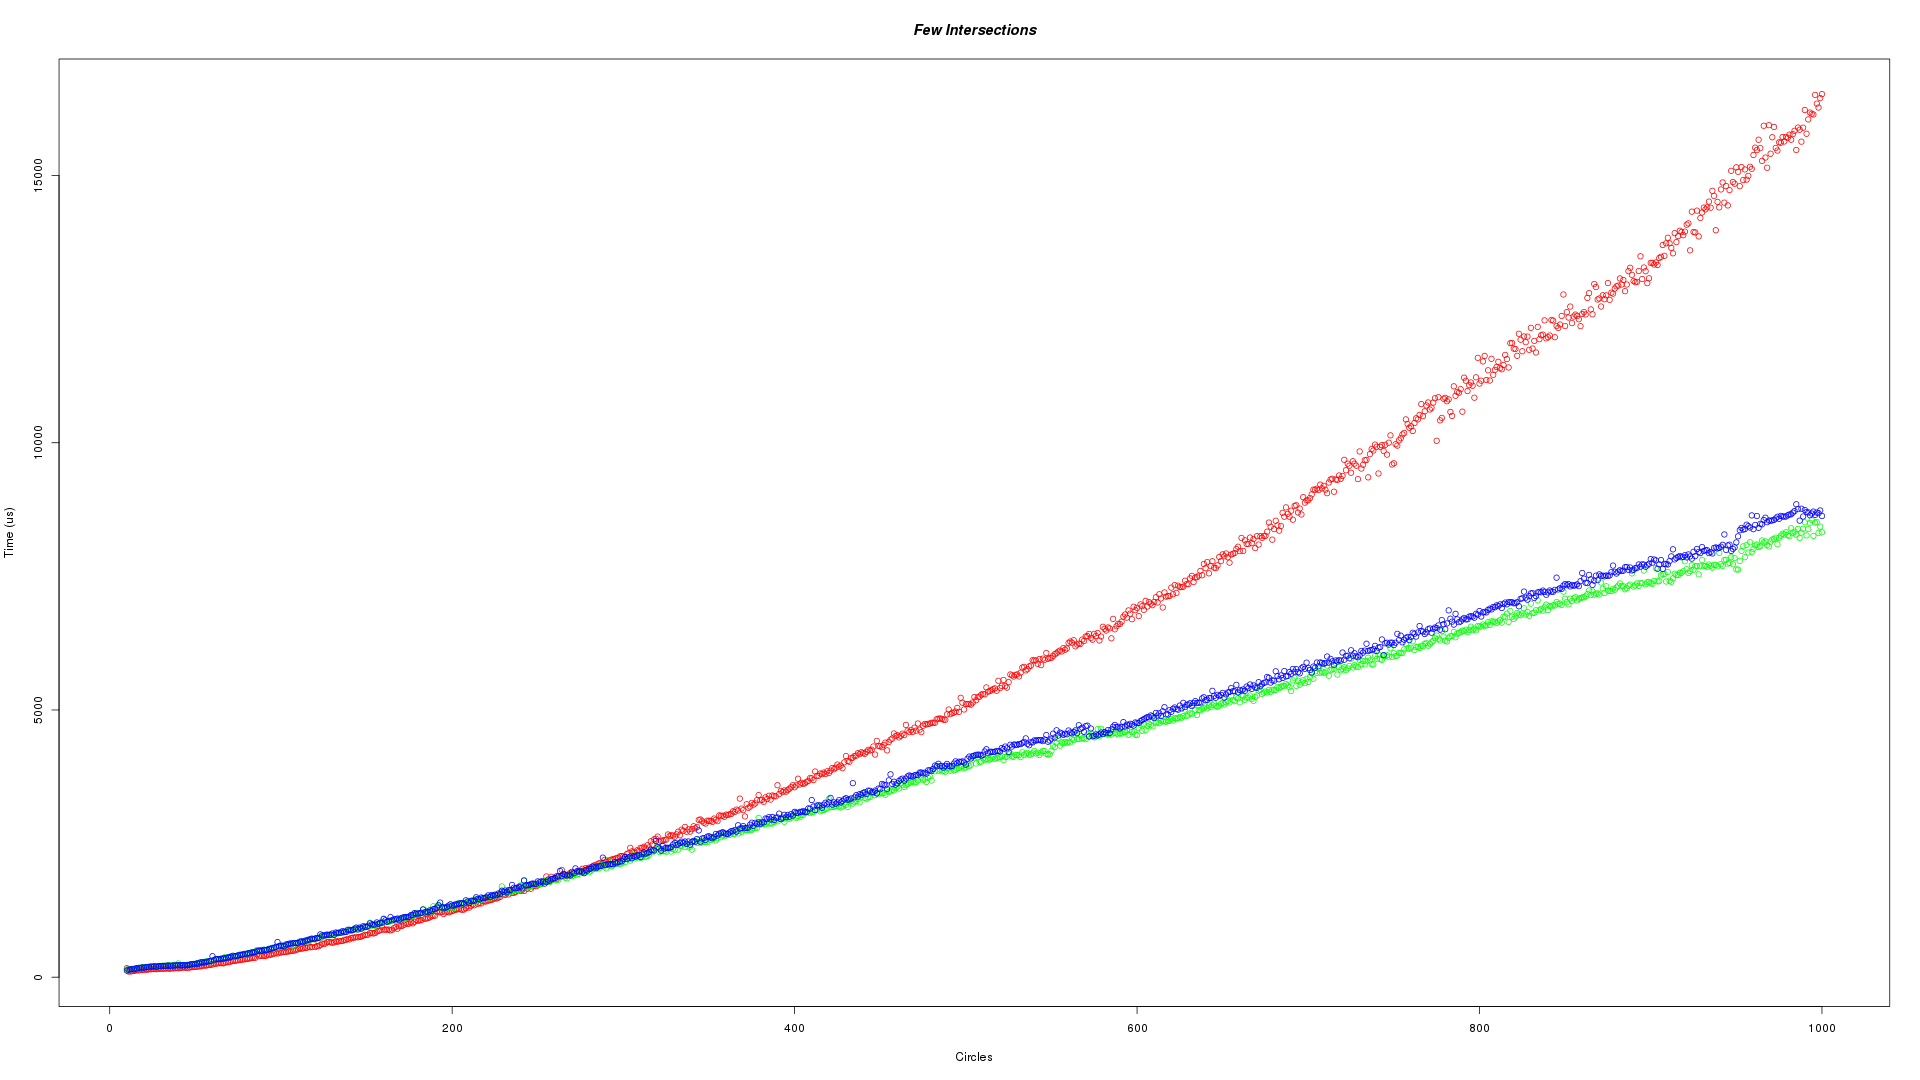
\includegraphics[width=\textwidth]{illustraties/fewIntersections.png}
  	\label{fig:few_intersections}
  	\caption{Uitvoeringstijden bij gevallen met weinig snijpunten.}
\end{figure}
In Figuur \ref{fig:few_intersections} zijn de resultaten uiteengezet van het eerste rauwe data-experiment. We zien dat het na\"ieve algoritme veel slechter presteert dan de andere twee. Het eerste algoritme wordt niet be\"invloedt door het aantal snijpunten, lijkt het.

\subsubsection{Gemiddeld Geval}
\begin{figure}[H]
	\centering
   	\includegraphics[width=\textwidth]{illustraties/averageCase.png}
  	\label{fig:average_case}
  	\caption{Uitvoeringstijden bij een gemiddeld geval snijpunten.}
\end{figure}
   
\subsubsection{Veel Snijpunten}
\begin{figure}[H]
   	\centering
   	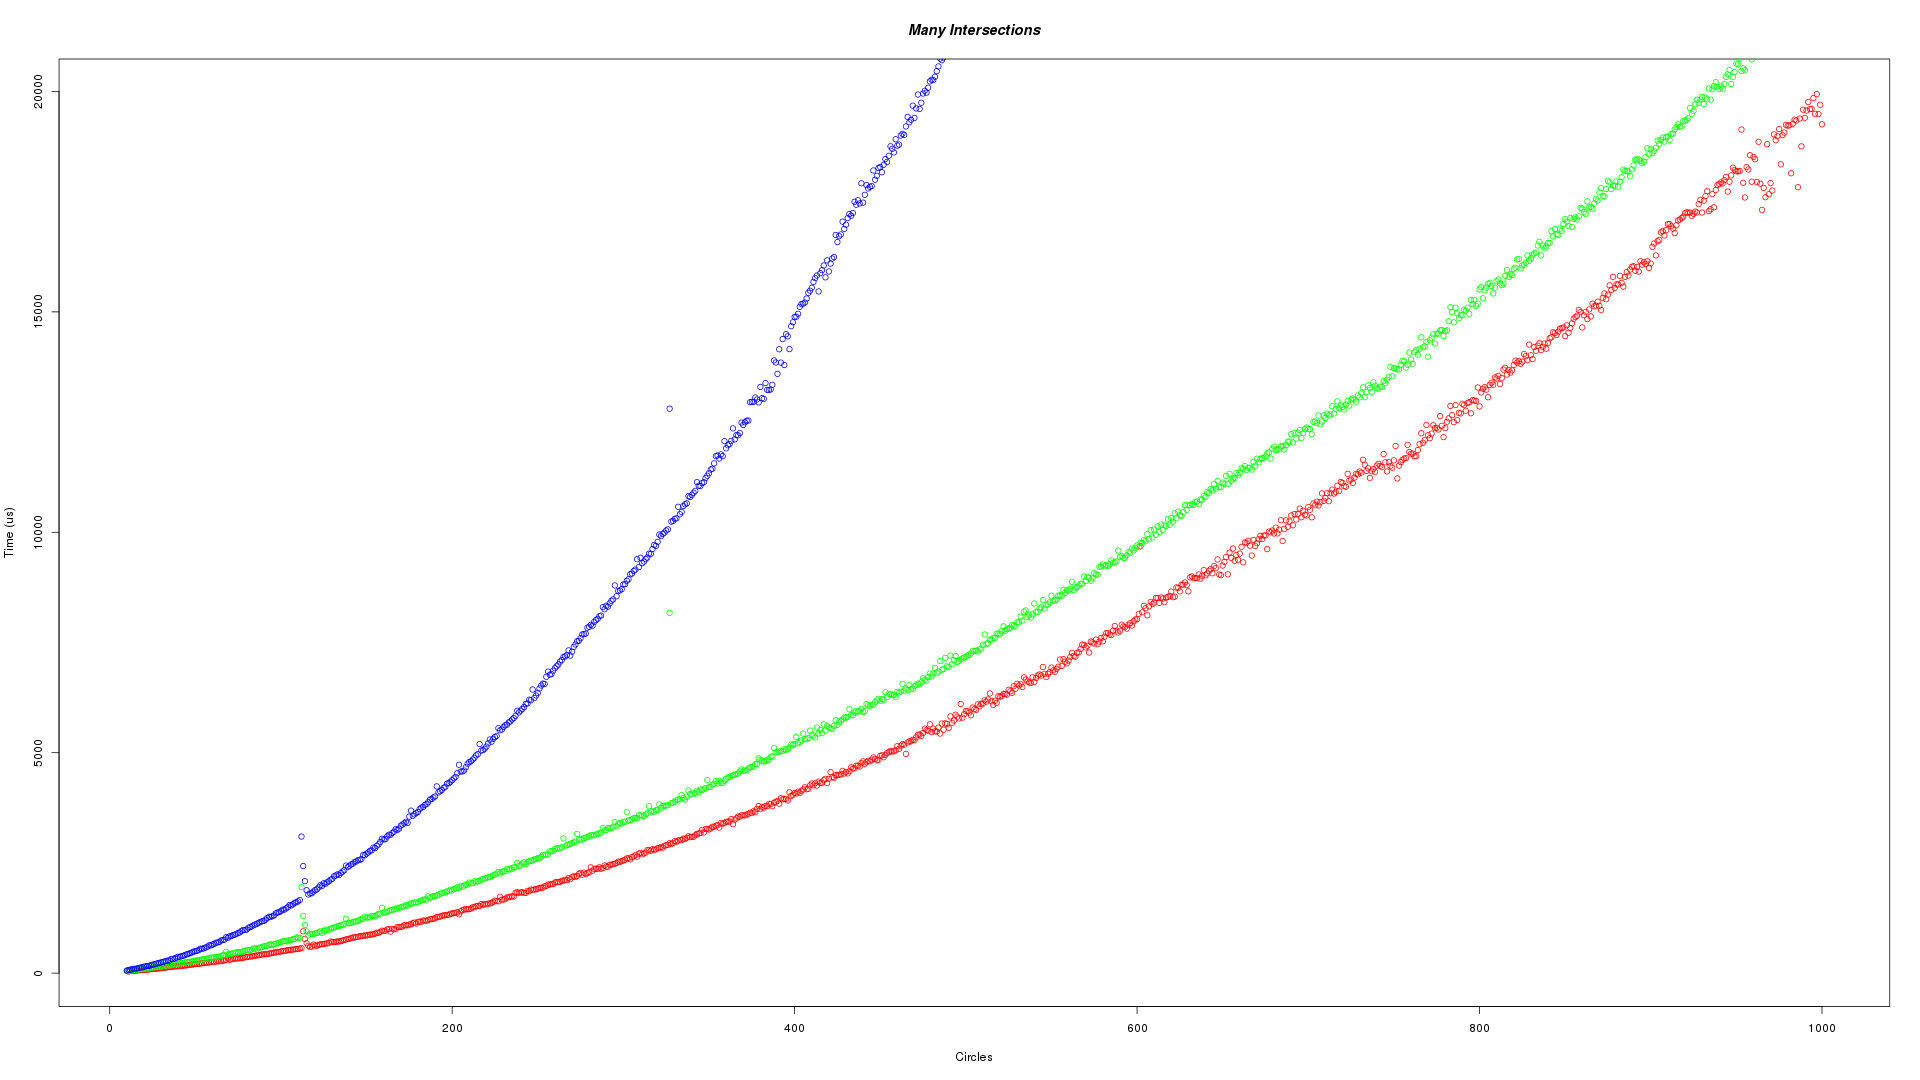
\includegraphics[width=\textwidth]{illustraties/manyIntersections.png}
   	\label{fig:many_intersections}
  	\caption{Uitvoeringstijden bij gevallen met relatief veel snijpunten.}
\end{figure}
In Figuur \ref{fig:many_intersections} zijn de resultaten uiteengezet van het tweede rauwe data-experiment. We zien dat algoritme \'e\'en hier beter presteert dan de andere twee. Algoritme twee en drie moeten dezelfde snijpunten berekenen maar hebben te kampen met enige `overhead'.

\subsubsection{3D plot}
\begin{figure}[H]
   	\centering
   	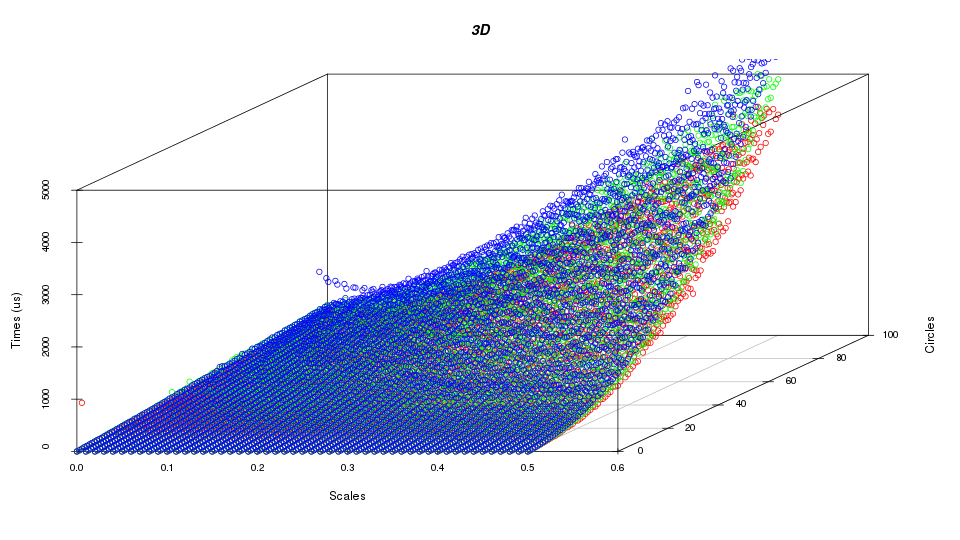
\includegraphics[width=\textwidth]{illustraties/3DScatter.png}
	\label{fig:3d}
  	\caption{Een 3D grafiek van de uitvoeringstijden in functie van de scalering en het aantal cirkels}
\end{figure}
De resultaten van het laatste rauwe data-experiment staan in Figuur \ref{fig:3d}.
Het is duidelijk dat algoritme \'e\'en ongeveer evenveel tijd nodig heeft onafhankelijk van de scalering van de stralen. We zien bovendien dat algoritme drie slechter presteert dan algoritme \'e\'en bij grote scaleringen en beter bij kleine scaleringen.

\subsection{Doubling Ratio}
\todo{doubling ratio resultaten uitleggen}
\subsubsection{Naief}
\begin{table}[H]
\[
\begin{array}{|c||ccccccc|}
\hline 
& 20 & 40 & 80 & 160 & 320 & 640 & 1280\\
\hline \hline 
0.000 & 3.4 & 3.9 & 4.6 & 4.2 & 4.3 & 4.3 & 4.2 \\ \hline 
0.001 & 3.2 & 4.3 & 4.2 & 4.9 & 4.1 & 4.3 & 4.2 \\ \hline 
0.500 & 3.5 & 4.0 & 4.5 & 4.8 & 4.9 & 4.8 & 5.0 \\ \hline 
1.000 & 3.4 & 4.2 & 4.5 & 4.7 & 5.3 & 5.3 & 5.3 \\ \hline 
\end{array}
\]


\label{fig:doublingratio_1}
\caption{Doubling ratio 1}
\end{table}
Figuur \ref{fig:doublingratio_1} toont de resultaten van het doubling ratio exeriment voor algoritme \'e\'en. Het is makkelijk te zien dat de ratio zal convergeren naar $4$ voor een groot aantal cirkels. Dit bovendien onafhankelijk van de scalering van de stralen.

\subsubsection{Kwadratisch}
\begin{table}[H]
\[
\begin{array}{|c||ccccccc|}
\hline 
& 20 & 40 & 80 & 160 & 320 & 640 & 1280\\
\hline \hline 
0.000 & 1.8 & 2.3 & 2.2 & 2.3 & 2.1 & 2.2 & 2.1 \\ \hline 
0.001 & 2.0 & 2.4 & 2.1 & 2.5 & 2.2 & 2.3 & 2.6 \\ \hline 
0.500 & 3.1 & 3.9 & 4.2 & 4.3 & 5.1 & 5.2 & 5.1 \\ \hline 
1.000 & 3.7 & 4.3 & 4.0 & 4.7 & 5.5 & 5.1 & 5.4 \\ \hline 
\end{array}
\]


\label{fig:doublingratio_2}
\caption{Doubling ratio 2}
\end{table}
In Figuur \ref{fig:doublingratio_2} de resultaten van het doubling ratio experiment voor algoritme twee. Voor kleine scaleringen van de straal zien we dat de ratio rond $2.2$ schommelt. Wanneer er weinig snijpunten zijn is dit algoritme dus inderdaad beter dan kwadratisch.
Voor grote scaleringen schommeld de ratio rond $4$ zoals verwacht van een kwadratisch algoritme.

\subsubsection{Linearitmisch}
\begin{table}[h]
\[
\begin{array}{|c||ccccccc|}
\hline 
& 20 & 40 & 80 & 160 & 320 & 640 & 1280\\
\hline \hline 
0.000 & 2.2 & 2.2 & 2.2 & 2.3 & 2.2 & 2.1 & 2.2 \\ \hline 
0.001 & 2.1 & 2.2 & 2.2 & 2.3 & 2.8 & 1.8 & 2.4 \\ \hline 
0.500 & 3.3 & 3.4 & 4.1 & 4.4 & 5.2 & 5.2 & 5.0 \\ \hline 
1.000 & 3.4 & 4.0 & 4.2 & 4.6 & 5.5 & 5.1 & 5.1 \\ \hline 
\end{array}
\]


\label{fig:doublingratio_3}
\caption{Doubling ratio 3}
\end{table}
In Figuur \ref{fig:doublingratio_3} staan de resultaten van het laatste doubling ratio experiment.
We zien dat de ratio rond 2.2 schommelt voor kleine scaleringen.
Dit komt overeen met onze voorspellingen.
Bij kleine $S$ zal de uitvoeringstijd van het algoritme namelijk linearitmisch groeien.
Bij grote scaleringen schommelt de ratio boven $4$ zoals verwacht van een $O(N^2\log(N))$ algoritme.

